\documentclass{ctuthesis}
%\usepackage{float}
\usepackage{csquotes}
\usepackage{multirow}
\usepackage{booktabs}
\usepackage{tabularx}
\newcommand{\tabitem}{~~\llap{\,\begin{picture}(-1,1)(-1,-3)\circle*{3}\end{picture}\ }~~}
\usepackage{array}
\usepackage{ragged2e}
\newcolumntype{P}[1]{>{\RaggedRight\hspace{0pt}}p{#1}}

\ctusetup{
	doctype-czech = {Bakalářská práce},
	xfaculty = F3,
	mainlanguage = czech,
	titlelanguage = czech,
	title-english = {Create REST service for conversion from LaTeX to PDF},
	title-czech = {Vytvoření REST služby pro konverzi LaTeX souborů do PDF},
	department-czech = {Katedra počítačů},
	author = {TADEÁŠ KYRAL},
	supervisor = {Ing. LUKÁŠ ZOUBEK},
	supervisor-address = {Katedra ekonomiky, manažerství a humanitních věd},
	fieldofstudy-czech = {Softwarové inženýrství a technologie},
	subfieldofstudy-czech = {žádné},
	keywords-czech = {PDF, LaTeX, PDF, Moodle, CourseWare, Web service, REST, Java EE},
	keywords-english = {PDF, LaTeX, PDF, Moodle, CourseWare, Web service, REST, Java EE},
	%front-specification = true,
	%specification-file = {}, % PDF s tvym zadanim prace
	day = 2,
	month = 11,
	year = 2018,
}

\ctuprocess

\addto\ctucaptionsczech{%
	\def\supervisorname{Vedoucí}%
}

\setcounter{tocdepth}{1}

% Podekovani
\begin{thanks}
	V první řadě bych chtěl poděkovat svému vedoucímu JMENO za příjemnou spolupráci a cenné rady při naších konzultacích. Dále bych chtěl poděkovat mé rodině a kamarádům, kteří mě
	při psaní této práce podporovali.
\end{thanks}

% Prohlaseni
\begin{declaration}
	Prohlašuji, že jsem předloženou práci vypracoval samostatně, a že jsem uvedl veškerou použitou literaturu.
	
	V Praze, \ctufield{day}.~\monthinlanguage{title}~\ctufield{year}
\end{declaration}


% Abstrakt v anglictine
\begin{abstract-english}
	Text follows...
\end{abstract-english}


% Abstrakt v cestine
\begin{abstract-czech}
	Práce pojednává o návrhu a vývoji webové služby pro konverzi LaTeXu do PDF, pro uživatele v Moodle a CourseWare. Doplněk má uživatelům usnadnit práci s LaTeXovými soubory přímo skrze portál Moodle, bez potřeby stahování a kompilace na svém stroji. Byla naimplementována služba na server a následně byla zapojena do provozu. Uživatelům portálů se usnadnila práce s LaTeX soubory. 
\end{abstract-czech}


\begin{document}
	\maketitle

	\chapter{Úvod}
LaTeX patří v akademickém prostředí mezi velmi oblíbené typografické systémy a je hojně využíván ke psaní skript a odborných prací. Mnoho akademiků využívá LaTeX i k vytváření materiálů pro studenty, primárně v oblasti matematiky, jelikož nabízí jednoduché nástroje ke psaní vzorců. Hlavním zdrojem materiálů pro studenty jsou portály Moodle a CourseWare, kam vyučující dokumenty nahrávají a můžou je tam i upravovat. Nynější editor podporuje jenom řádkové příkazy a není schopen zpracovat celý LaTeX dokument natož s více zdrojovými soubory. Tento stav mnoha učitelům nevyhovuje, protože by chtěli svoje dokumenty upravovat a přímo kompilovat v prohlížeči bez potřeby je stahovat a následně zase nahrávat. 

Práce se dělí na čtyři hlavní části. Nejdříve proběhne seznámení s potřebnou teorií a technologiemi, dále budou specifikovány požadavky na službu z čehož se najdou již podobné existující řešení a porovnají se s požadavky. Následně se přistoupí k návrhu samotné aplikace.


\section{Cíle práce}
Hlavním cílem bakalářské práce je poskytnout konverzi LaTeX souborů do PDF pro uživatele Moodle a CourseWare. Čehož bude dosaženo implementováním webové služby, která bude schopna komunikovat pomocí REST Api. K tomu vedoucí jednotlivé dílčí cíle jako analýza existujících řešení, návrh, implementace a v neposlední řadě testování. 

	   
  \chapter{Teorie a technologie}
  V této části si přiblížíme technologie potřebné k návrhu a vývoji webové služby specifikované v zadání práce. Postupně budou vysvětleny všechny zásadní pojmy, které pomůžou čtenáři doplnit znalosti.
  
  \section{REST}
	Representational state transfer (dále jen REST) je architektura pro komunikaci  mezi distribuovanými systémy. Termín zavedl R. T. Fielding ve své disertační práci\cite{restThesis}, kde toto rozhraní bylo taktéž popsáno a vymezeno. Mimo jiné stanovil i těchto 5 základních pravidel, které by měly být dodrženy, aby se aplikace mohla nazývat RESTful\cite{rest}:
	\begin{itemize}
		\item Klient-Server(Client-Server) - Toto omezení staví na principu oddělení zodpovědností (Separation of Concerns), nebo-li je klientská část starající se o uživatelské rozhraní a serverová část přistupující k databázi. Zlepšuje škálovatelnost sytému a zjednodušuje použitelnost na různých platformách.
		\item Bezestavovost(Stateless) - Každý požadavek musí přenášet všechna související data, server totiž neuchovává žádné informace o nynějším spojením a každý požadavek bere jako nový.
		\item Keš(Cache) - Data přenášená v odpovědi mohou být označená jako kešovatelná, tudíž si je klient může uložit a kdykoliv použít znova.
		\item Jednotné rozhraní(Unified interface) - Základem tohoto omezení je princip HATEOAS (Hypermedia As The Engine Of Application State), které říká, že klient nepotřebuje znát pravidla komunikace dopředu a data musí obsahovat odkazy na další data v aplikaci. Jasně definovaná adresa zdroje (např. URI), reprezentace přenášených dat (např. HTML), typ média (např. JSON)
		\item Vrstvený systém(Layered system) - Přidáním vrstev se aplikace, kde každá vrstva je izolovaná a může komunikovat jenom se soudějícími vrstvami, zpřehlední a zlepší se její škálovatelnost.
	\end{itemize}	
	Nejčastějším typem protokolu využívající tuto architekturu je Hypertext Transfer Protocol(HTTP). Pomocí třech hlavních metod GET, PUT, POST, DELETE v požadavku poslaného z klienta server buď odpovídajíce vrátí požadovaná data, přijme data poslané v těle a například uloží do databáze, nebo data vymaže. 

\section{Java EE}
	Tato platforma je rozšířením standardní Javy SE a je primárně určená pro vývoj webových aplikací. Nabízí  Java EE potřebuje ke svému fungování aplikační server, který se stará o požadavky, komunikuje s databází apod. Mezi hlavní pojmy patří bean, container, component, dependency injection, 
	

\section{PDF}
	Portable Document Format(dále jen PDF), jak už název napovídá jedná se o formát dokumentů, jejichž hlavním cílem je poskytování nazávislosti na platformě. Soubor se skládá ze čtyř komponent: 
	\begin{itemize}
		\item Objekty(Objects) - Základní jednotka celého souboru např. Pole, Čísla, Řetězce znaků. Jednotlivé objekty se popisují množinou znaků, která je definována lexikálními konvencemi.
		\item Struktura objektů(File Structure) - Soubor je rozdělen na čtyři části: 
			\begin{figure}
				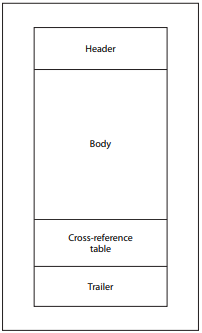
\includegraphics[scale=0.8]{Untitled}
				\centering
				\caption{Struktura objektů}
			\end{figure}
			\begin{itemize}
				\item hlavička - identifikuje verzi PDF
				\item tělo - obsahuje použité objekty, které reprezentují obsah dokumentu
				\item tabulka odkazů - obsahuje odkazy na objekty v podobě počtu bytů od začátku souboru, kvůli náhodnému přístupu bez potřeby číst celý soubor
				\item závěrečná sekce - udává pozici tabulky odkazů a speciálních objektů
			\end{itemize}
		\item Struktura dokumentu(Document Structure) - Popisuje hierarchickou strukturu objektů v těle dokumentu.
		\item Content stream - Objekt v kterém se nacházejí instrukce k vykreslování grafických elementů. 
	\end{itemize}
	
 \section{LaTeX}
	Vychází z typografického sázecího systému TeX, který popisuje Pavel Satrapa ve své knize \cite{latex}: \enquote{\textit{Patří do rodiny tak zvaných značkovacích jazyků (markup languages) a dal by se zjednodušeně charakterizovat jako programovací jazyk pro sazbu textů. Jeho základním vstupem je textový soubor, který obsahuje jak sázený dokument, tak příkazy ovlivňující sazbu. Určité znaky mají přiřazen speciální význam a jejich prostřednictvím jsou v textu odlišeny řídicí konstrukce. Typickým příkladem je zpětné lomítko, jímž začínají příkazy.}}
	
	LaTex je rozšíření TeXu o balíček přednastavených řídících konstrukcí. Hlavní cílem těchto systému je jednoduchost pro psaní matematických a jiných vzorců. Ovšem je také velmi oblíben kvůli silné možnosti upravovat dokumenty ke svému zalibení.
	
	Příkazy a text se píše do souborů s příponou tex tyto soubory musí dodržovat jistou stromovou strukturou. V kořenu stromu je jeden hlavní soubor, do kterého jsou vnořovány další. To napomáhá přehlednosti velkých dokumentů a také používání již vytvořených. Následně se musí všechny soubory zkompilovat do výstupního souboru, který může být například ve formátu PDF nebo DVI. 

\section{FURPS+}
	Vychází z klasifikace požadavků FURPS(\textbf{F}unctionality, \textbf{U}sability, \textbf{R}eliability, \textbf{P}erformance, \textbf{S}upportability) s kterou přišel Robert Grady v roce 1992. Roku 1999 Jacobson at el rozšířili specifikaci o znaménko "+", které přidává požadavky a omezení na design, implementaci, rozhraní a hardware. 
	
	\begin{itemize}
		\item Funkční požadavky
			\begin{itemize}
				\item Functionality - Požadavky popisujicí všechny hlavní prvky produktu i důležité aspekty z pohledu architektury např. lokalizovaný systém pro více jazyků.
			\end{itemize}
		\item Nefunknční požadavky
			\begin{itemize}
				\item Usability - Zaměřuje se na uživatelskou přívětivost nejenom samotné aplikace, ale i dokumentace apod., týkající se estetiky a konzistence
				\item Reliability - Spolehlivost systému v podobě času fungování, správnosti fungování a četnosti výpadků
				\item Performance - Vypovídá o výkonnosti systému, jak rychle dokáže zpracovávat požadavky, nastartovat atd.
				\item Supportability - Popisuje testovatelnost, škálovatelnost, konfigurovatelnost...
				\item Design - Omezení na design systému např. požadavek na relační databázi
				\item Implementation - Specifikuje typ prorgamovacího jazyku, platformu apod.
				\item Interface - Komununikace s externímy systémy
				\item Physical - Definuje požadavky na hardware, na kterém daný software poběží i co se týče velikosti
			\end{itemize}
	\end{itemize}
	
	Toto rozdělení nám pomáhá identifikovat požadavky. Přispívá k vyšší kvalitě systému a snižuje pravděpodobnost přehlédnutí funkcionality.
 
	 \chapter{Analýza}
 
 
 \section{Požadavky} \label{requirements}
 Nyní představíme požadavky kladené na aplikaci. Ty jsou buď požadované zadávajícím nebo odvozené z potřeb, ke kterým bude služba používána.Ale i z omezení plynoucích z prostředí v jakém bude provozována, v tomto případě pro fakultu státní vysoké školy, jmenovitě Fakulta elektrotechnická, ČVUT. \\
 Za pomoci metody FURPS+ rozdělíme požadavky a omezení na funkční a nefunkční. 
 
 \subsection{Funkční požadavky} \label{functional}
 \begin{table}[H]
 	\begin{center}
 		\begin{tabular}{ p{4cm} P{0,7cm} P{7,9cm} }
 			\textbf{Typ} & \multicolumn{2}{l}{\textbf{Požadavky}} \\
 			\midrule[0,15em]
 			Funkčnost 
 			&\multicolumn{2}{l}{\tabitem Webová služba s REST rozhraním pro komunikaci} \\
 			&\multicolumn{2}{l}{\tabitem Umět přijmout požadavky a soubory}\\
 			&\multicolumn{2}{P{7,6cm}}{\tabitem Zkompilování \LaTeX\ souborů s požadovaným nastavením do PDF}\\
 			&\multicolumn{2}{l}{\tabitem Uložení PDF a jeho poskytnutí}\\	
 			&\multicolumn{2}{l}{\tabitem Uživatel může zvolit tyto nastavení:}\\
 			&&\tabitem {\small Přidat vodoznak na každou stranu PDF}\\
 			&&\tabitem {\small Nakonec souboru přidat stránku s předem stanoveným obsahem}\\
 			&&\tabitem {\small Výsledný soubor PDF bude chráněný}\\
 			&&\tabitem {\small Výsledný soubor PDF nebude kopírovatelný nebo tisknutelný}\\
 		\end{tabular}
 	\end{center}
 	\caption{Funkční požadavky}
 	\label{tab:errors}
 \end{table} 
 Služba ma jediný a specifický účel, z toho plyne menší množství funkcionalit. 
 
 \subsection{Nefunkční požadavky}
 
 \begin{table}[H]
 	\begin{center}
 		\begin{tabular}{ p{4cm} P{8,6cm} }
 			\textbf{Typ} & \textbf{Požadavky} \\
 			\midrule[0,15em]
 			Použitelnost & \tabitem Dokumentace k rozhraní na swagger\footnote{https://swagger.io/}\\
 						& \tabitem Přístup skrz REST Api, pouze s tokenem\\
 			\midrule		
 			Spolehlivost & \tabitem Služba není kritická\\
 						& \tabitem Uptime 95\% času\\
 						& \tabitem Ochrana proti špatnému vstupu\\
 						& \tabitem Autorizace pomocí tokenů\\
 			\midrule
 			Výkon & \tabitem Zvládnutí obsloužení desítky požadavků najednou\\
 						& \tabitem Ukládání výsledných dokumentů po dobu jednoho měsíce\\
 						& \tabitem Maximální doba tvorby dokumentu 5 minut\\	
			\midrule
			Podporovatelnost & \tabitem Služba může být rozšířena o kompilování samotného TeXu a může podporovat vytváření i jiných formátů z \LaTeX u\\	
			\midrule
			Implementace & \tabitem Platforma - Java EE\\
						& \tabitem Komunikace - REST Api\\
						& \tabitem Operační systém - Ubuntu nebo CentOS\\
			\midrule
 			Rozhraní & \tabitem Komunikuje s Moodle a CourseWare, tyto portály posílají data\\
 			\midrule
 			Fyzické & \tabitem Musí být provozováno na serverech ČVUT\\
 	\end{tabular}
 	\end{center}
 	\caption{Nefunkční požadavky}
 	\label{tab:errors}
 \end{table}
 
 Důvody některých požadavků nemusejí být úplně jasné, proto je zmíníme.
 \begin{itemize}
 	\item Platforma - Je požadováno prostředím vývoje, kde Java EE je hlavní platforma. Tudíž je zajištěna podpora. 
 	\item Operační systém - Také vyžadováno z pohledu podpory, zmíněné systémy jsou na serverech, kde bude služba nasazena nejčastěji používány a tudíž správci tyto systémy znají.   
 	\item Služba není kritická - Poskytuje funkčnost, která nijak neovlivňuje základní funkcionality určených portálů. 
 	\item Musí být provozováno na serverech ČVUT - Jelikož aplikace bude pracovat s dokumenty a popřípadě i informacemi, spojenými s pracovníky školy, je potřeba tyto data chránit a uchovávat na vlastních serverech z důvodu GDPR.
 \end{itemize}
 
 Z tabulky je vidět, že služba není nijak kritická a působí jenom jako doplněk do výše zmíněných portálů. Musí ovšem splňovat vyšší bezpečnostní nároky zapříčiněné prostředím v jakém se bude používat. 

\section{Existující řešení}
Na základě stanovených požadavků v minulé kapitole přejdeme k analýze již existujících řešení. Momentálně uživatelé Moodle mohou vkládat do svých souborů řádkové příkazy, což není úplně dostačující a nesplňuje to požadavky. Samozřejmě se dají používat pro vytváření PDF z \LaTeX\ souborů kompilátory, které si můžete stáhnout a používat lokálně. To ovšem není předmětem této práce, a proto se podíváme na webové služby, které více odpovídají potřebám a požadavkům. Pár vybraných si představíme.  

\subsection{OverLeaf}
Placená služba\footnote{https://www.overleaf.com} pro tvorbu \LaTeX\ dokumentů, která umožňuje i používání zadarmo s některými omezeními. Je velmi oblíbená hlavně kvůli hezkému prostředí pro tvorbu dokumentů a jejich správu. Také nabízí výhody pro určité zájmové skupiny, nejzajímavější vzhledem k tématu této práce je předplatitelská služba OverLeaf Commons \footnote{https://www.overleaf.com/for/universities}. Ta poskytuje sdílené prostředí se všemi výhodami pro zaměstnance a studenty univerzity. Ale jako všechny ostatní služby je i tato placená, ovšem není jisté jestli ji poskytují pro všechny univerzity a ani za jakých podmínek.

\subsection{BlueLaTeX}
Open-source služba\footnote{http://www.bluelatex.org/} pro kompilaci LateX souborů. Kompilovat můžete na jejich serveru nebo nabízejí kód pro spuštění na vlastním. Kromě samotné serverové implementace je k dispozici i webový klient. Vše je pouze zatím v Beta verzi a samotní tvůrci varují před možnými nedostatky a problémy. Na jejich oficiálních stránkách je poslední aktivita z roku 2015 a zdá se, že tento projekt už není aktivní. Hlavním lákadlem je souběžná spolupráce více lidí na jednom dokumentu a také možnost provozovat server lokálně. 

\subsection{ScienceSoft}
Starší služba\footnote{http://sciencesoft.at/latex/index?lang=en}, která mimo kompilace \LaTeX\ souborů vložených přes webový prohlížeč poskytuje i jiné rozhraní pro poskytnutí souborů a to jmenovitě REST Api a SOAP. Jak bylo řečeno, tak tato služba je starší, tudíž pro kompilaci používá zastaralý TexLive 2008 a její vývoj není aktivní.

\subsection{ShareLaTeX}
Velmi podobný BlueLaTeXu, tedy open-source\footnote{https://github.com/sharelatex/clsi-sharelatex} nabízející jimi hostovanou verzi nebo lokální verzi pro vlastní potřebu, obě verze obsahují mnoho funkcí včetně grafického prostředí pro uživatele. Pod jménem ShareLaTeX se vyskytuje jenom výše zmíněné, ovšem společně s OverLeaf také spravují službu Pro\footnote{https://www.overleaf.com/for/enterprises}, která je určená pro firmy, ale i univerzity. Ta se pyšní možností nasazení na vlastních serverech, správou uživatelů, podporou a zabezpečením. 

\subsection{Porovnání}
Každé z těchto řešení ma své problémy, ať už že je zastaralé a neaktualizované nebo nesplňující zanalyzované požadavky(sekce \ref{requirements}). Do první skupiny patří ScienceSoft a BlueLaTex, kde první z jmenovaných ani neposkytuje kód pro implementaci na lokálním serveru a druhý je v nedodělaném stavu, což může vést k nefunkčnosti a bezpečnostním rizikům. Služba Overleaf Commons nesplňuje stejný požadavek jako řešení od ScienceSoft, ale nabízí zajímavé prostředí pro vytváření a správu \LaTeX\ dokumentů pro studenty i zaměstnance, o čemž by univerzita mohla popřemýšlet. Nejnadějnější možností se zdá být ShareLaTeX, který poskytuje k použití i jenom backendovou část pro kompilaci \LaTeX\ a komunikaci, ale celý je implementovaný v CoffeeScriptu, což si rozporuje s požadavkem na implementaci, kde je Java EE. 

\section{Kompilátory}
Nejdůležitější částí celé aplikace bude kompilátor, který bude provádět kompilaci \LaTeX\ souborů, ale může poskytnout i podporu pro operace s výsledným PDF. Tyto operace vycházejí ze stanovených funkčních požadavků(sekce \ref{functional}). Jelikož kompilace bude probíhat na serveru s Linuxovým operačním systémem nebudeme zahrnovat do srovnání kompilátory pro Windows.

\subsection{MikTeX}
MikTeX \footnote{https://miktex.org} je velmi oblíbený hlavně na operačním systému Windows, díky příjemné instalaci a kvůli možnosti doinstalovávat balíčky \enquote{on-the-fly}, neboli za běhu. Ale je poskytován i mimo jiné pro Linux a to například pro potřeby této práce v zajímavé verzi \enquote{Just enough TeX}. Tato instalace obsahuje jen to nejnutnější, tedy bez zbytečných balíčků navíc. Je vyvíjen jediným programátorem, který se stará o celou distribuci, což je do budoucnosti lehce rizikové z pohledu udržitelnosti. Podporované Linuxové operační systémy jsou např. nejnovější Ubuntu a Debian.

\subsection{TeXLive}
TeXLive je kompilátor spravovaný skupinou přispěvatelů, kteří ho udržují. Existují dvě různé cesty jak TeXLive\footnote{https://www.tug.org/texlive/pkginstall.html} nainstalovat a od toho se odvíjí správa balíčků. Verze Native TeX Live a distribuce přímo pro daný operační systém. Liší se ve počtu balíčků po instalaci a způsobu jejich aktualizací. V Native verzi probíhají aktualizace pomocí TeX Live Manager nebo-li tlmgr, jinak se o to stará samotný operační systém. Pokud si vyberete Native je možno si i zvolit schéma, které určuje množství balíčků např. scheme-basic obsahuje jenom to nejnutnější. Podporuje skoro všechny Linuxové distribuce.

\subsection{Porovnání} \label{compilator}
Oba kompilátory jsou si velmi podobné a liší se jenom v drobnostech, některé z nich už byly nastíněny v jejich popisech. Jedním z důležitých aspektů je velikost instalace, tedy i s balíčky, v této kategorii nabízejí oba to samé. K tomuto se váže práce s balíčky, kde už je jiná situace a to kvůli jasné výhodě MikTeXu stahovat balíčky během běhu. Něco podobného jde dosáhnout i v TexLive, ale je nutno použít externí skripty, což může mnohem více ovlivňovat rychlost kompilace. 
Rozdíl je také ve správě samotných kompilátorů, kde MikTeX je náchylnější k výpadkům aktualizací nebo celkově zastavení vývoje, kvůli jedinému člověku, který se o něj stará. To může vést i k dalším problémům, co se týče bezpečnosti a podpory.

	  
  	\chapter{Vlastní řešení}  

V této části navrhneme podobu vlastního řešení problému specifikovaného v předchozích kapitolách. Návrh by měl nabízet jednoduché a vyhovující řešení vycházející ze stanovených požadavků a cílů. 

\section{Návrh}

Cílem práce je poskytnout konverzi \LaTeX\ souborů do PDF, čehož bude dosaženo pomocí webové služby. Tato služba bude poskytovat svoje rozhraní a funkcionalitu portálům Moodle a CourseWare. Jedná se o jednoduchou aplikaci s jediným účelem, tedy kompilace \LaTeX\ souborů do PDF. Tudíž není potřeba složité databáze, ale stačí pouze SQLite\footnote{https://www.sqlite.org/}, což je velmi odlečená verze klasických SQL databází, která ukládá data přímo do souboru v souborovém systému, kam bude ukládán i výsledný soubor PDF. 

\subsection{Platforma}
Na základě požadavků bude aplikace postavena na Java EE, což je platforma pro vývoj webových aplikací rozšiřující standardní Javu SE. Oproti ní poskytuje některé zásadní techniky navíc, jednu si tedy představme. 
\par
\textbf{Vkládání závislostí} (dependency injection) umožňuje objektu používat jiné objekty bez potřeby ho zatěžovat jejich vytvářením. Objekty, které můžeme takto vkládat, se nazývají beany a právě o jejich vytváření a zánik se stará Contexts and Dependency Injection (dále jen CDI) kontejner.
\\[12pt]
\par
Dále je potřeba specifikovat aplikační server. Ten poskytuje pro webové aplikace běhové prostředí, tedy zajišťuje správu databázových spojení apod. Na základě zkušeností je vybrán open-source Payara, který staví na GlassFish, oproti němu poskytuje častější aktualizace a opravy chyb. 

\subsection{Architektura}
Architektura popisuje z jakých částí se aplikace skládá, jak mezi sebou tyto části komunikují a jakým způsobem procházejí informace a požadavky aplikací. Při navrhování architektury je potřeba zvážit několik věcí, například rozšířitelnost, modularizaci, odezva a složitost. 
\par
Nejpoužívanšjší architekturou u webových aplikací je klient-server architektura s n vrstvami, která aplikaci rozděluje na n fyzických médií a n vrstvá architektura, která označuje n logických celků.\footnote{V anglických zdrojích se používají výrazy N-Tier Client-Server architecture a N-Layered architecture, kde tier znamená to samé jako layer, tudíž vrstva} Nejčastěji jsou obě architektury 3 vrstvé, tedy rozdělení je následující: prezentační, aplikační a databázová vrstva. Ovšem služba, kterou se zabýváme v této práci nemá uživatelské rozhraní a vystavuje jenom určité API, tudíž odpadá prezentační vrstva. Ani neobsahuje databázový server, zůstává tedy jenom aplikační fyzická vrstva, což z naší služby dělá jedno-vrstvou klient-server aplikaci. Zbývá ještě vyřešit logickou architekturu, kde se budeme držet také zavedeých postupů, ale zbavíme se prezentační vrstvy a zůstane nám 2-vrstvá architektura obsahující byznys logiku a přístup k databázi.  

\begin{figure}[H]
	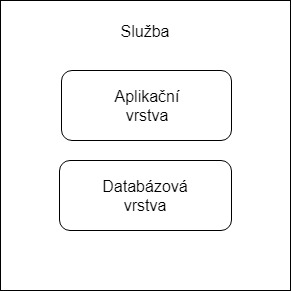
\includegraphics[scale=0.7]{architecture}
	\centering
	\caption{Architektura}
	\label{fig:arch}
\end{figure}

\subsection{Komunikace}
Pro komunikaci mezi klientem a serverem je vybráno REST Api. Poskytuje jednoduché rozhraní, se kterým je schopen komunikovat jakýkoliv systém pouze na základě znalosti struktury požadavků a odpovědí. Posílání zpráv bude postaveno nad protokolem HTTP pomocí GET a POST metod. Na obrázku \ref{fig:seq} je zobrazena komunikace mezi serverem a klientem. 

\begin{figure}[H]
	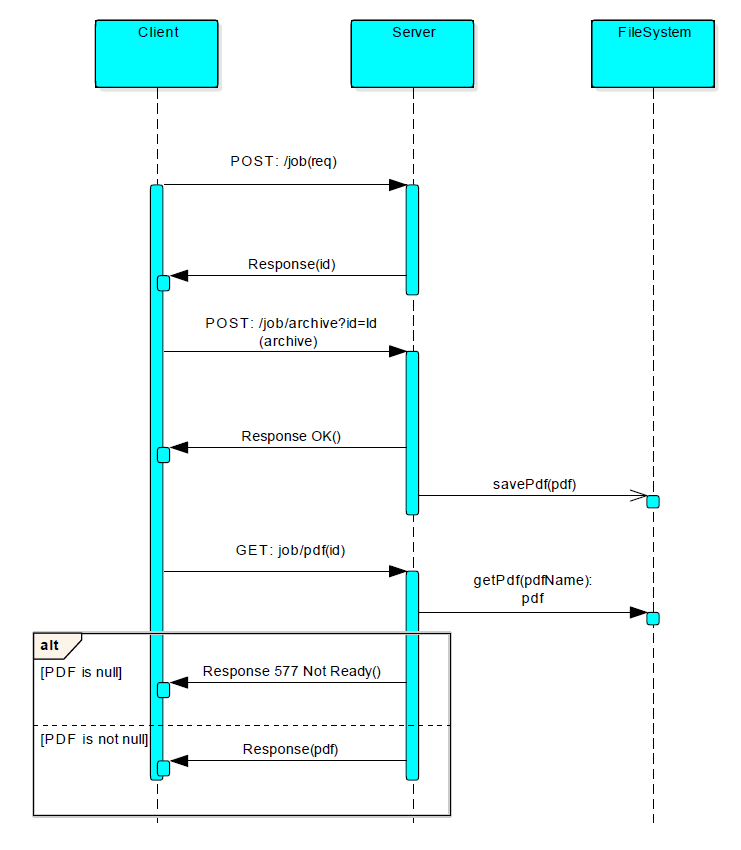
\includegraphics[width=0.9\textwidth]{diagram}
	\centering
	\caption{Sekvenční diagram}
	\label{fig:seq}
\end{figure}

Kompletní dokumentace k rozhraní se nachází na swagger\footnote{https://app.swaggerhub.com/apis/Tadky/Thesis/1}. Na ukázku vypíšeme alespoň používané zdroje:
\begin{itemize}
	\item \textbf{POST} {\ttfamily /job} - Slouží k předání požadavků na výsledné PDF.
	\item \textbf{POST} {\ttfamily /job/archive?id=<jobId>} - Musí obsahovat zip archiv s potřebnými soubory pro kompilaci.
	\item \textbf{GET} {\ttfamily /job/pdf?id=<jobId>} - Vrací výsledné PDF, pokud už je hotové.
	\item \textbf{HEAD} {\ttfamily /job/pdf?id=<jobId>} - Odpověď obsahuje pouze hlavičku, která informuje o stavu PDF
	\item \textbf{GET} {\ttfamily /info} - Slouží k získání informací ohledně serveru, tedy verze kompilátoru, operačního systému, zbývajícího volného místa na disku
\end{itemize}
Všechny tyto zdroje navíc obsahují parametr\footnote{Typ parametru, který se posílá v samotné URL daného dotazu ve formě klíč=hodnota} token, který zajišťuje autentizaci. Ta je rozebrána v další sekci.

\subsection{Zabezpečení}
Zabezpečení bude zavedeno jenom v minimální míře pomocí statických tokenů, které budou mít dané portály pro sebe k dispozici. Vzhledem k povaze dat není nutné používat OAuth\footnote{Protokol pro autentizaci a autorizaci aplikací.} server, jehož implementace by byla značně nad rámec mé práce. Tokeny budou sloužit k autentizaci portálů, jímž budou tokeny vygenerovány a předány jejich správcům. Každá zpráva poslaná na server bude obsahovat token, který se bude ověřovat oproti tokenu uloženém v properties\footnote{Soubor v němž jsou data uspořádány klíč = hodnota} souboru. Token bude posílán v parametru dotazu v otevřené formě. 

\subsection{Kompilace}
Pro vytvoření PDF je nutné příslušně zkompilovat celý \LaTeX\ projekt. Pro úspěšnou kompilaci je potřeba, aby kompilátor měl k dispozici všechny balíčky, které jsou použity v projektu. Jsou tři způsoby, jak toho docílit.
\begin{enumerate}
	\item Stáhnout všechny balíčky již při instalaci kompilátoru
	\item Nainstalovat čistý kompilátor
		\begin{enumerate}
			\item Stáhnout několik balíčků a jenom ty se budou používat
			\item Získávat balíčky podle potřeby za běhu
		\end{enumerate}
\end{enumerate}
První možnost je zbytečná z důvodu mnoha nepoužívaných balíčků a velikosti na disku. Druhá možnost nabízí dvě podmožnosti, kde volba s přednastavenými balíčky vytváří omezení pro uživatele a tím pádem je může odrazovat od používání. Nejvíce vhodná se zdá poslední možnost, která eliminuje všechny neduhy předchozích, tím pádem je i zvolena.
\par
Na základě porovnání kompilátorů (sekce \ref{compilator}) z předchozí kapitoly je zvolen MikTeX, který poskytuje vše potřebné a nabízí vhodné funkcionality pro téma této práce např. doinstalovávání balíčku za běhu. Bude nainstalován ve verzi \enquote{Just enough TeX}, tudíž nebude obsahovat žádné balíčky. Ty se právě budou doinstalovávat až na požadavek při kompilaci.

\subsection{PDF úpravy}
Jelikož jsou kladeny požadavky na výsledný soubor PDF a bohužel kompilátory tyto úpravy nepodporují, je potřeba použít jiný nástroj, který bude umožňovat měnit soubor podle požadavků. Nejvíce vhodný se zdá PDFtk\footnote{https://www.pdflabs.com/tools/pdftk-server/}, který je pod GPL\footnote{Poskytuje svobodu šíření, provozování a upravování daného software.} licencí a nabízí vše potřebné. Tedy po zkompilování do PDF se za pomoci výše zmíněné aplikace aplikují požadavky, které byly obdrženy od klienta.

\subsection{Server}
V této fázi návrhu máme už všechny potřebné informace, aby mohl být zvolen operační systém a stanoveny požadavky na server. Jsou známy dvě omezující podmínky kladené na systém. První vychází z požadavků: operační systém musí být Debian nebo CentOS. Druhou určuje kompilátor. Jelikož byl zvolen MikTeX, který je podporován na Debian a Ubutnu, volba je jednoznačná. Na základě průniku je vybrán nejnovější Debian, tedy verze 9 s označením \enquote{stretch}. 
\par
Je také potřeba stanovit velikost diskového pole potřebného pro fungování. Jelikož nejvíce místa budou zabírat balíčky a potažmo výsledné pdf, budeme vycházet hlavně z těchto údajů. Přibližná velikost všech balíčků obsažených v plné verzi kompilátoru je zhruba 4GB, což bylo zjištěno na základě testovací instalace. Dále je potřeba odhadnout velikost všech PDF, které musí server uchovávat po dobu jednoho měsíce, v jeden moment. Horní odhad pro počet vytvořených PDF za den je 30 a pro velikost souboru je 10MB. Tedy na konci měsíce se může očekávat velikost cca 10GB. Tedy celkové požadované místo je 15GB.  
 



  

	\begin{center}
		\textit{R = (A $\lor$ B $\lor$ C $\lor$ D)}
	\end{center}
 
 	\begin{figure}[H]
 		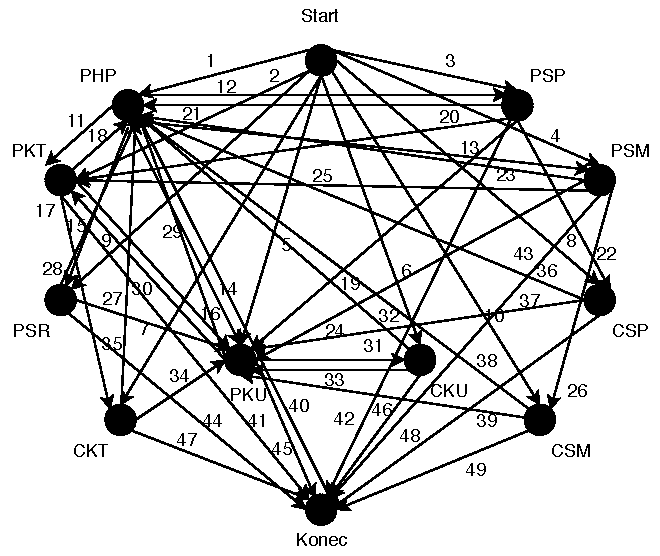
\includegraphics[width=0.9\textwidth]{process_app}
 		\caption{Vizualizace průchodu aplikací}
	 \end{figure}
	
	\chapter{Implementace}

	\chapter{Závěr}
	Text follows
	
	\bibliographystyle{acm}
	\bibliography{ctubib}
	
	\appendix

\chapter{Seznam zdrojů}

\medskip
\bgroup \leftskip=5.5em

\begin{itemize}
	
	\item Obrázek \ref{fig:pdf} -- Převzato z dokumentace PDF\cite{pdf} 25. 11. 2018.
	\item Obrázek \ref{fig:seq} -- Vytvořeno autorem 30. 12. 2018.
	\item 
	
\end{itemize}

\par\egroup
	
	\appendix

\chapter{Seznam zkratek}

\medskip
\bgroup \leftskip=5.5em

\begin{description}
	
	\item[FURPS] -- Functionality, Usability, Reliability, Performance, Supportability
	
	\item[GDPR] -- General Data Protection Regulation
	
	\item[HTTP] -- Hypertext Transfer Protocol
	
	\item[API] -- Aplikační rozhraní
	
	\item[CW] -- CourseWare
	
	\item[\TeX] -- Typografický sázecí systém
	
	\item[\LaTeX] -- Lamport \TeX\ - balík maker pro \TeX
	
	\item[PDF] -- Portable Document Format
	
	\item[REST] -- Representional State Transfer
	
	
	

\end{description}

\par\egroup
	
	



	
\end{document}